\PassOptionsToPackage{quiet}{xeCJK}
\documentclass{cumcmthesis}
\setCJKmainfont{SimSun.ttf}[AutoFakeBold]
\usepackage{etoolbox}
\usepackage{float}
\BeforeBeginEnvironment{tabular}{\zihao{-5}}
\usepackage[numbers,sort&compress]{natbib}  % 文献管理宏包
\usepackage[framemethod=TikZ]{mdframed}  % 框架宏包
\usepackage{url}  % 网页链接宏包
\usepackage{subcaption}  % 子图宏包
\newcolumntype{C}{>{\centering\arraybackslash}X}
\newcolumntype{R}{>{\raggedleft\arraybackslash}X}
\newcolumntype{L}{>{\raggedright\arraybackslash}X}

\title{全国大学生数学建模竞赛论文模板}  % 论文标题
\tihao{B}  % 题号
\baominghao{202527001171}  % 报名号
\schoolname{西安交通大学}  % 学校
\membera{李冬阳}  % 队员a
\memberb{曹芷维}  % 队员b
\memberc{朱韵桐}  % 队员c
\supervisor{陈磊}  % 指导老师
\yearinput{2025}
\monthinput{9}
\dayinput{7}
\begin{document}


\maketitle

\begin{abstract}
本文围绕碳化硅外延层厚度的测量这一问题,以\textbf{红外干涉法}为主要手段,针对双光束干涉和多光束干涉的不同情景分别建立数学模型并设计厚度求解方案,旨在制定一套科学、准确、可靠的碳化硅外延层厚度测试标准。


\textbf{对于问题一,}基于光在外延层-衬底只发生一次反射的\textbf{双光束干涉}的情景,我们利用干涉的基本原理,由几何关系推得光程差,并利用\textbf{斯涅尔折射定律}和干涉条件下的相位差所满足的关系式,建立起红外光谱的波长、外延层的折射率和红外光的入射角等参数与外延层厚度相关联的数学模型,为后续外延层厚度的计算奠定模型基础。

\textbf{对于问题二,}基于问题一所建立的数学模型,设计了外延层厚度的算法,并将附件1和附件2的数据可视化处理,利用\textbf{傅里叶变换}提取周期。同时结合\textbf{菲涅尔公式}等算得外延层厚度,通过模型的检验和计算过程的分析,验证模型的可靠性与准确性。

\textbf{对于问题三,}


最后,



\keywords{关键词\quad  关键词\quad  关键词\quad  关键词 \quad 关键词}
\end{abstract}

\section{问题重述}
\subsection{问题背景}
碳化硅(SiC)作为第三代半导体材料,因其优异的物理与电学性能,在高温、高压、高频等极端工况下展现出巨大潜力。外延层厚度是SiC器件设计与制造中的关键参数,直接影响器件的核心性能指标。因此,建立一套无损、高精度、可重复的外延层厚度测试标准,对产业界与学术界均具有重要意义。

红外干涉法是目前主流的无损检测手段,利用SiC外延层与衬底层折射率不同的特性,发射红外光线并接受来自外延层与衬底层的反射光线,确定SiC外延层的厚度。其基本原理是:红外光在SiC外延层表面与外延/衬底界面分别发生反射,两束反射光因光程差产生干涉条纹,通过分析反射光谱,间接计算外延层的厚度。
%%%%%%%%%%%%%%%%%%%%%%%%%%%%%%%%%%%%%%%%%%%%%%%%%%%%%%%%%%%%% 

\subsection{问题要求}

\textbf{问题1}  
在仅考虑一次反射与透射的简化情形下,建立由红外光谱反演SiC外延层厚度的通用数学模型。

\textbf{问题2}  
利用问题一中我们提出的模型,利用附件1、2中的实测数据计算SiC外延层厚度,并分析结果的可靠性。

\textbf{问题3} 

%%%%%%%%%%%%%%%%%%%%%%%%%%%%%%%%%%%%%%%%%%%%%%%%%%%%%%%%%%%%% 

\section{问题分析}
\subsection{问题一分析}
红外干涉法测量碳化硅外延层厚度的核心在于双光束干涉现象。当红外光以特定入射角照射样品时,在外延层表面与衬底界面分别产生一束反射光。这两束光因传播路径不同形成光程差,其大小取决于外延层厚度、材料折射率及入射光波长。光程差导致两束光在探测器处发生相位叠加:当相位相同时呈现相长干涉(反射率极大值),相位相反时则发生相消干涉(反射率极小值)。

另外,外延层折射率与波长有关。不同波长的入射光在材料中经历不同的折射行为,这使得光程差成为波长的复合函数。这一特性导致反射光谱呈现周期性振荡现象——反射率随波长变化形成明暗交替的干涉条纹,即反射率函数呈现出波动的特性。条纹的振荡频率与外延层厚度直接关联:厚度越大,光谱振荡越密集;厚度越小,振荡越稀疏。

因此,反射率振荡曲线的特征提取是厚度计算的关键。通过分析震荡曲线的特性可建立振荡周期特征与外延层厚度的定量映射关系,即所求数学模型

\subsection{问题二分析}	
对于问题二,

\subsection{问题三分析}
对于问题三,


%%%%%%%%%%%%%%%%%%%%%%%%%%%%%%%%%%%%%%%%%%%%%%%%%%%%%%%%%%%%% 

\section{模型假设}

为简化问题,本文做出以下假设:

\begin{itemize}[itemindent=2em]
\item 假设1 材料均匀:假设外延层是厚度均匀、光学性质各向同性的介质,且其上、下表面是光滑的理想平行平面。
\item 假设2 折射率假设:假设入射介质为空气,其折射率 $n_0$ 恒定为 1。

\item 假设3 光源假设:入射的红外光可视为理想的单色平行光。
\end{itemize}

%%%%%%%%%%%%%%%%%%%%%%%%%%%%%%%%%%%%%%%%%%%%%%%%%%%%%%%%%%%%% 

\section{符号说明}
\begin{table}[H]
\centering
% 修改列数为 4 列,将格式改为 CCCC
\begin{tabularx}{\textwidth}{CCCC}%这里写表格的列数、对齐方式
\toprule
符号    & 说明    & 单位    \\
\midrule
$d$     & 外延层厚度 & $\mu m$ \\
$n$     & 折射率 & 无单位 \\
$\theta$ & 入射角 & 度($^\circ$) \\
$\theta_2$ & 折射角 & 度($^\circ$) \\
$\Delta d$ & 光程差 & $\mu m$ \\
$\lambda$ & 波长 & $\mu m$ \\
$\tilde{\nu}$ & 波数 & $cm^{-1}$ \\
\bottomrule
\end{tabularx}
\label{tab:符号说明}
\end{table}

\section{问题一的模型的建立和求解}
\subsection{模型建立}
\subsubsection{双光束干涉的基本原理}
光具有波动性,当两列(或更多)频率相同、振动方向相同、相位差恒定的相干光波在空间相遇时,会发生干涉现象。
反射光1为入射光在空气-外延层界面直接反射的光,反射光2为入射光在透射过空气-外延层界面,在外延层-衬底界面反射,然后透射过空气-外延层界面射出的光,两光束实际为同一光源发出,相干性良好。

由于反射光2比反射光1多走一段光程,这个固定的光程差导致两束光之间产生了一个恒定的相位差, 
当光束由空气(光疏介质)进入外延层(光密介质)反射光有 π 的相位突变(半波损失),虽然我们无法判断当光由外延层进入衬底时是否会发生半波损失,但在两种情况下两束光由于半波损失造成的附加的相位差是一定的。综上,光程差和半波损失共同造成的相位差是恒定的,又因为两束光具有高度相关性,所以当两束光在空间中相遇时会发生干涉现象。

由于外延层的折射率会随着波长的改变而变化,所以当入射光的波数改变时,两束光之间的光程差会发生改变,进而。若光程差为半波长的偶数倍,此时发生干涉相长,反射光增强而产生明纹;若光程差为半波长的奇数倍,此时发生干涉相消,反射光减弱而产生暗纹(需解释为啥)。综上,随着波数的增加,会形成明暗相间的干涉条纹,进而体现在反射率-波数函数曲线的振荡周期性变化,其中函数的极大值对应明纹,极小值对应暗纹。

由于半波损失带来的相位差是一定的,不会对函数曲线的振荡周期产生影响,因此不会影响本文所建立模型中外延层厚度的计算。所以后文中两束光的相位差简化为只由光程差所造成的相位差。
\subsubsection{数学模型建立}
\begin{figure}[htbp]
	\centering
	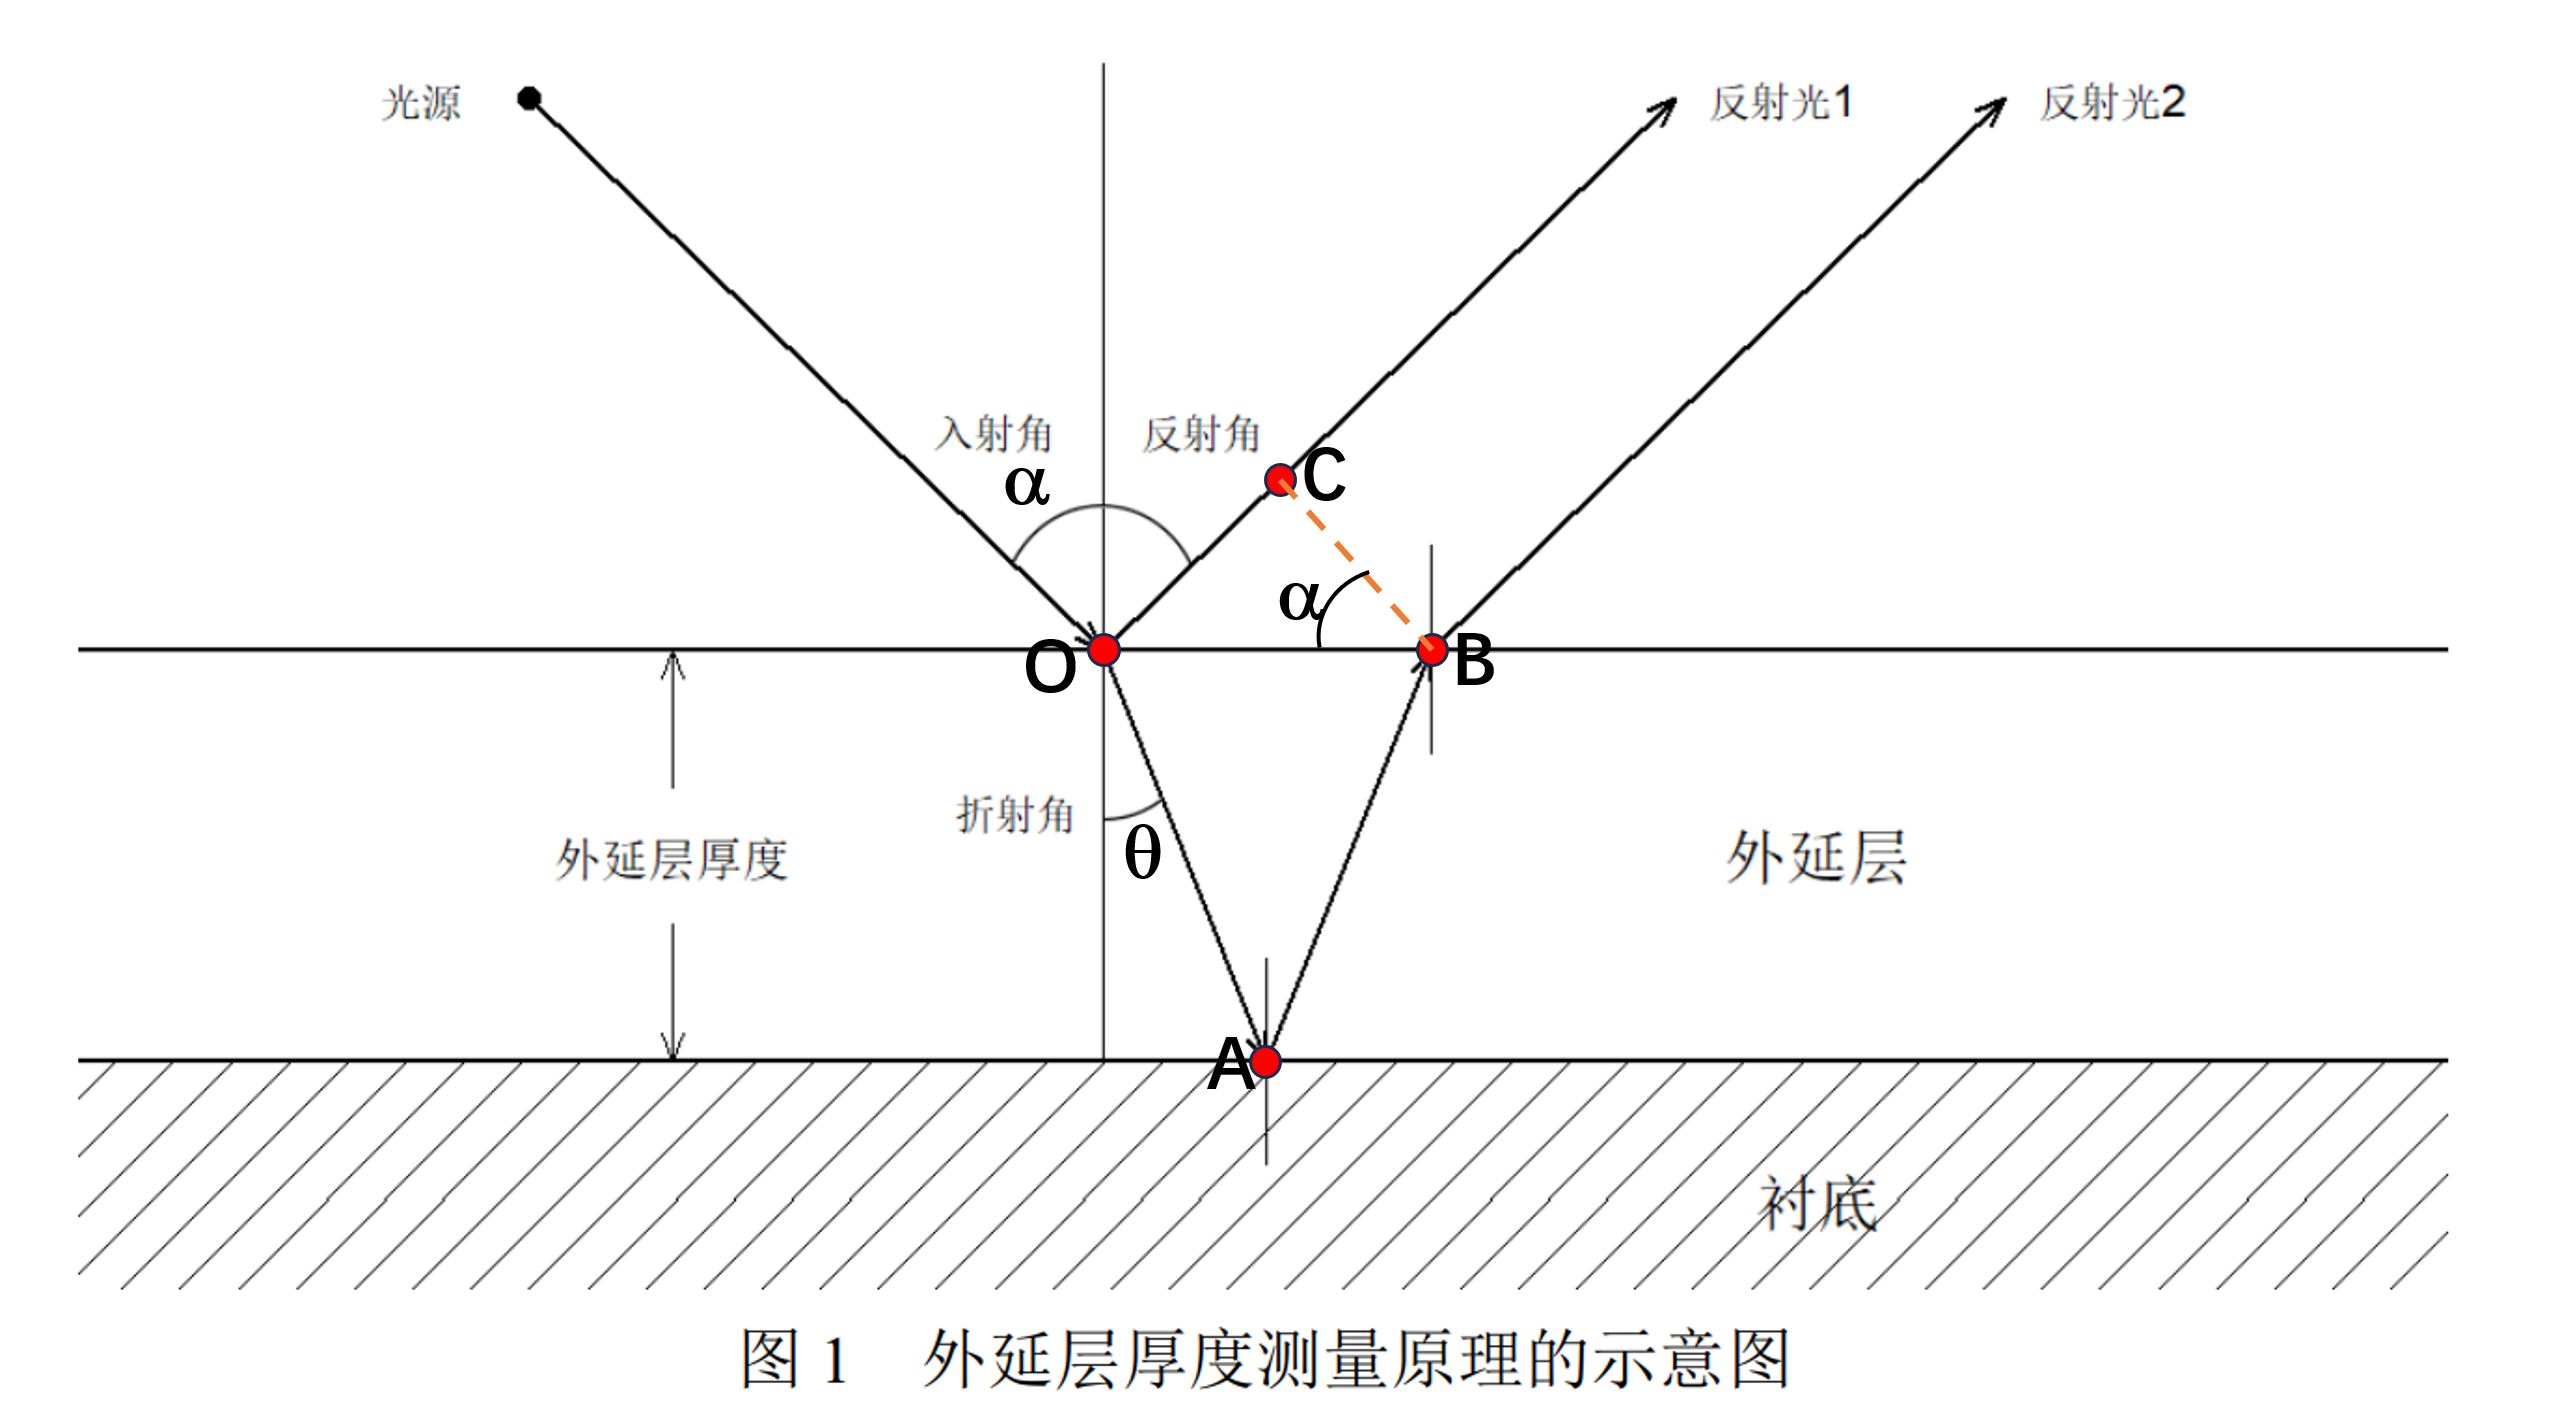
\includegraphics[width=0.8\textwidth]{q1_1.png}
	\caption{}
	\label{fig:q1_1}
	\end{figure}
由图中几何关系易得等式(1)(2)(3)
\begin{gather}
\Delta L = n_2 \cdot(AO + AB) -n_1\cdot OC\\
AB = AO = \frac{d}{n_2 \cdot\sin\theta } \\
OC = OB \cdot \tan\alpha 
\end{gather}
斯涅尔折射定律:
\begin{gather}
n_1 \sin \alpha = n_2 \sin \theta 
\end{gather}
联立(1)(2)(3)(4)解得:\\

$$\Delta L = 2\cdot d \cdot \sqrt{n_2^2 - \sin \alpha^2} $$  \\
相位差:
\begin{gather}
	\Delta \phi = 2\pi \frac{\Delta L}{\lambda}
\end{gather}
干涉相长-“明纹”情况下双光束的相位差所满足的条件:
\begin{gather}
	\frac{2\pi}{\lambda}\Delta L = 2\cdot m\cdot \pi  \quad (m=1,2,3,\ldots)
\end{gather}
干涉相消-“暗纹”情况下双光束的相位差所满足的条件:
\begin{gather}
	\frac{2\pi}{\lambda}\Delta L = (2\cdot m + 1 )\cdot \pi \quad (m=1,2,3,\ldots)
\end{gather}
在实际观测中,我们发现SiC外延层的折射率会随着波长的变化而变化,在第二问的求解中,我们将会考虑波长对于折射率的影响。在此处,我们认为波长变化不大时,折射率可以视为常数。因此我们的结论是(带初相位$\varphi$):
\begin{equation}
	d = \frac{m (\lambda + \varphi)  }{2\sqrt{n_2^2 - \sin \alpha^2}}
\end{equation}
通过观测数据的两个峰值的间距,或者波谷(把波长换算为波数)。有:
\begin{equation}
2v_1d\sqrt{n_2^2 - \sin \alpha^2} = m
\end{equation}
\begin{equation}
2v_2d\sqrt{n_2^2 - \sin \alpha^2} = m+1
\end{equation}
(9)(10)作差得:
\begin{equation}
2(v_2-v_1)d\sqrt{n_2^2 - \sin \alpha^2} = 1
\end{equation}
令$
|v_1 - v_2| = \Delta T
$
,并整理得到外延层厚度d的表达式为:\begin{equation}
d = \frac{1}{2 \Delta T \sqrt{n_2^2 - \sin \alpha^2}}
\end{equation}
综上所述:厚度d由波数差$\Delta T$,折射率$n_2$,以及入射角$\alpha$确定。
	 
	\section{第二问}
	\subsection{模型建立}
	\begin{equation}
	d = \frac{1}{2 \Delta T \sqrt{n_2^2 - \sin \alpha^2}}
	\end{equation}
	由第一问可以得到模型,我们采用什么方法求T,采用什么方法求n,大致思路
	\subsection{数据可视化与预处理}
	通过matplot库函数,画出附件一和附件二的图像。我们明显看到,附件一二在波数在500-1000有着明显的突变。通过查资料我们得知,这部分可以删除:这里把源资料拿过来(标注是抄的,最后要优化一下语句降低重复率)
	\subsubsection{提取周期}
	傅里叶变换可以将时域信号转换为频域信号,通过分析频域特征,能够有效推测出数据中的周期成分。利用傅里叶变换就可以清晰地找到这些周期信号,进而分离出整体趋势和周期扰动。
输出:平均周期: 252.629
	\subsubsection{计算折射率}
	题目明确提到外延层的折射率通常不是常数,它与掺杂载流子的浓度、
红外光谱的波长等参数有关。由于附件1和附件2使用的是同一块块碳化硅晶圆片,故可以假设载流子浓度一定,折射率的主要影响因素为红外光谱的波长。菲涅耳公式描述了光在不同介质分界面上的反射和折射的振幅、相位等关系。能够结合光的反射、折射等光学现象的观测数据来得到折射红外光谱的波长等参数有关。由于附件1和附件2使用的是同一块块碳化硅晶圆片,故可以假设载流子浓度一定,折射率的主要影响因素为红外光谱的波长。菲涅耳公式描述了光在不同介质分界面上的反射和折射的振幅、相位等关系。能够结合光的反射、折射等光学现象的观测数据来得到折射率。
	\begin{equation}
	\begin{split}
	\frac{K}{K + 1} = &\frac{1}{2}\bigg[ \left( \frac{n_1 \cos\theta_i - \sqrt{n_2^2 - n_1^2 \sin^2\theta_i}}{n_1 \cos\theta_i + \sqrt{n_2^2 - n_1^2 \sin^2\theta_i}} \right)^2 + \\
	&\left( \frac{n_2^2 \cos\theta_i - n_1 \sqrt{n_2^2 - n_1^2 \sin^2\theta_i}}{n_2^2 \cos\theta_i + n_1 \sqrt{n_2^2 - n_1^2 \sin^2\theta_i}} \right)^2 \bigg]
	\end{split}
	\end{equation}
这里详细解释一下,下面这两张图是如何得出的
第零步:由文献,在1500/cm之上sic为透明介质,不吸收光线第一步:计算反射率 R 根据您已知的反射光与折射光的光强比,计算出光线在介质分界面的反射率 R。(这一段我来写)第二步:选择相应的菲涅尔公式我们认为光线为非偏振光,使用公式计算
\subsection{计算d}
们提取出了附件1函数的周期性变化的周期,通过(什么方法)得到
最优 T
通过最优T我们根据公式 ,我们带入附件1求出的T,附件1的角度15度,以及相对应的折射率最终计算出d的结果为:没计算出来

	
\subsection{验证}
从题目得知,附件一和附件二是基于同一块材料所做的两次实验,两次实验的不同在于入射角角度不同。所以,理论上讲,我们使用附件一和附件二计算出来的d是相同的。基于这个物理事实,我们选择使用使用附件二,用处理附件一的方法处理附件二,得出d值,然后比较二者的相对偏差。如果d的相对偏差在可接受程度之内,说明我们的模型具有可靠性。第二,我们还通过,求附件一和附件二的d的均值,然后反代入我们的模型,看最终数据与我们附件一和附件二的偏差程度,若偏差程度在可接受程度内,则说明模型具有一定的可靠性。第三,我们还可以进行灵敏度分析,进一步验证模型的可靠性。(这里思路有了,但还没想好)
\subsubsection{附件2验证}
我们把附件2按照上面的方法再次求出:
计算相对偏差率:
我们发现相对偏差率小于1


\subsubsection{灵敏度分析}
因为我们只有附件一和附件二的数据,所以我们不知道改如何进行灵敏度分析,这里我建议直接调教AI,让AI看看能不能进行灵敏度分析,如果能,直接赢了好吧。
\subsection{总结}
经过三次验证,我们的模型相对偏差多少,置信度区间多少,然后夸一夸,也可以再分析不足(比如在我们的折射率使用的就是一个周期内波数中点的折射率,这个会产生一部分的误差)

\section{问题三的模型的建立和求解}
\subsection{必要条件}
\textbf{光波的入射条件}:光波必须是从折射率较低的介质(如空气)垂直入射到外延层与衬底的界面上,才能保证反射和透射产生明显的干涉效应。

\textbf{多次反射}:光波必须在外延层和衬底的界面之间反射多次。每次反射后,光波的传播路径和相位都会发生变化,形成干涉图样。

\textbf{相位反转}:每次反射都会导致相位的变化,尤其是在光波从折射率较大的介质(外延层)反射回折射率较小的介质(空气或衬底)时,会发生半波相位反转。

\textbf{干涉条件}:为了形成清晰的干涉图样,光波的反射路径差必须满足干涉条件。具体为:
	\[
	2 n_2 d = m \lambda_2 \quad \text{或} \quad 2 n_2 d = \left( m + \frac{1}{2} \right) \lambda_2
	\]
	其中,\( n_2 \) 是外延层的折射率,\( d \) 是外延层的厚度,\( \lambda_2 = \frac{\lambda}{n_2} \) 是光在外延层中的波长,\( m \) 为整数,表示干涉级数。

\textbf{多光束干涉的贡献}:每一次反射的光波都会对总干涉图样产生贡献,干涉强度是各反射光波幅度和相位的叠加。

\textbf{外延层的折射率与波长}:外延层的折射率和光的波长对干涉效果有重要影响。不同的折射率和波长会改变光波传播的速度,从而影响干涉条纹的形成。

\subsection{模型求解}

\textbf{Step1:} 

\textbf{Step2:} 

\textbf{Step3:} 

\subsection{求解结果}

%%%%%%%%%%%%%%%%%%%%%%%%%%%%%%%%%%%%%%%%%%%%%%%%%%%%%%%%%%%%% 


\section{模型的分析与检验}

\subsection{灵敏度分析}

\subsection{误差分析}

%%%%%%%%%%%%%%%%%%%%%%%%%%%%%%%%%%%%%%%%%%%%%%%%%%%%%%%%%%%%%

\section{模型的评价}

\subsection{模型的优点}
\begin{itemize}[itemindent=2em]
\item 优点1
\item 优点2
\item 优点3
\end{itemize}

\subsection{模型的缺点}
\begin{itemize}[itemindent=2em]
\item 缺点1
\item 缺点2
\end{itemize}


\bibliographystyle{gbt7714-numerical}  % 引用格式
\bibliography{ref}  % 引用 ref.bib 文件,无需写 .bib 后缀


\newpage
%%%%%%%%%%%%%%%%%%%%%%%%%%%%%%%%%%%%%%%%%%%%%%%%%%%%%%%%%%%%%
%% 附录
\begin{appendices}
\section{文件列表}
\begin{table}[H]
\centering
\begin{tabularx}{\textwidth}{LL}
\toprule
文件名   & 功能描述 \\
\midrule
example.py & 问题一程序代码 \\
\bottomrule
\end{tabularx}
\label{tab:文件列表}
\end{table}

\section{代码}
\noindent example.py
\lstinputlisting[language=python]{code/example.py}
\end{appendices}

\end{document}
